\subsection{Assumptions on Implied Volatility}
Implied Volatility is a market view of future volatility. Market view can be influenced by a lot of systematic and idiosyncratic factors. Unlike other parameters like the current spot price, strike price, cost of carry and the time to expiration which can be directly observed, the volatility is not directly measurable because of its forward looking nature. The \cite{RateLab2008} remarks implied volatility as a measure of fear. Here the authors use the Merrill Lynch move index which measures the implied volatility in US Treasury options to signify how low levels of implied volatility often precedes sharp increases in volatility. Furthermore, implied volatility is influenced by the term structure. As options get closer to maturity, the expectation around implied volatility changes significantly as the uncertainty reduces. The focus of this analysis is on the short term options. The expiration of the options range from 31 days to 1 day. 
One thing that I need to confess upfront that I have completely ignored the term structure of implied volatility since I am working with short-term options that is the days left to expiry range from 1 to 31 days. This assumption can be defended on two grounds:
1. The short-term options have a low vega. That is, their price is not very sensitive to changes in implied volatility.    
2. Although the vega risk is low, the volatility of implied volatility is higher for short-term options. This means that you do not have a systematic shape of term structure of volatility when you are looking at options that are going to expire in few days.    
One of the key characteristics of volatility is that if you look at the volatility time series, the time series is usually stationary. This is a nice feature to have because this allows us to look directly at the distributions across different tickers and compare them. The volatility distribution also has very long and fat tail because of the clustering and sharp spikes. 


\subsection{Assumptions on Realised Volatility}
In order to construct the volatility risk premium for an option contract, we need to have an estimate of realised volatility. Has also explained in the preceding sections this can be done in several ways and hence it is not a trivial problem to solve. In this paper the estimate for the realised volatility would be the simple annualized standard deviation sampled at 5 minute intervals over a lookback period equal to the time left for expiration. 
Suppose an option contract is priced on 3rd February 2020 at 9:35 AM with an expiration on 21st February 2020. There are 18 days left for expiration. Hence the lookback period for the realized volatility would be from 07th January 2020 9:35 AM shifted back by 18 days that is 3rd February 2020 9:35 AM. We will calculate the simple standard deviation of five minute log returns in this lookback period and will annualize it. Also note that the US holidays and weekends are also taken into consideration while calculating the lookback horizon. Therefore, for every option contract that is priced in the market the realized volatility estimate is dynamically calculated by looking at the time that is left for expiration. This makes the realised volatility more representative of the specific time horizon relevant to the lifetime of the option which adds robustness to the analysis.

$$ RV= \sqrt{252 \times 6.5 \times 12} \times \sqrt{\frac{1}{N_{5m}-1} \sum_{i=1}^{N_{5m}} (r_i - \bar{r})^2} $$  

Here $N_{5m}$ is the number of 5 minute intervals in the lookback period.

\subsection{Moneyness or Delta?}
Another important insight to note here is that delta represents hedge ratio and not a probability. This assumption is especially crucial  Delta is usually interpreted as the probability of an option finishing in the money. However this is only true if the return distribution is balanced, which means the volatility is low.  When the price process of the underlying is volatile, such as cryptocurrency or biotechnology stocks, more delta will diverge from the probability (\cite{abdelmessih2020lessons}).  Intuitively, a 10\% out of the money option for a cryptocurrency is more likely to finish in the money than a 10\% out of the money option for a utility or retail stock. During the course of this paper, we will treat 50-Delta options as a standard for comparison across tickers. 


\subsection{Cost of Hedging}
Another important insight to note here is that the implied volatility also accounts for the hedging cost that the market maker uses to price the option. The market maker does not have any directional bias and it is apparent from the mathematical derivation using the Black Scholes formula that is also shown above that any cost above the intrinsic value of the option would reflect in the implied volatility. Furthermore the cost of hedging is directly dependent on the volatility and therefore it is incredibly difficult to distil implied volatility into pure volatility risk premium and the cost of hedging. The focus of this paper would be to look at the distributions of the volatility risk premium and skew and derive exploratory insights.

\subsection{Selection of Tickers}

We will laser this analysis on the call options for the following underlying tickers and asset classes. 
\begin{table}[h]
    \centering
    \begin{tabular}{|c|c|c|}
        \hline
        \textbf{Ticker} & \textbf{Category} & \textbf{Trade Name} \\
        \hline
        FXY & FX & CurrencyShares Japanese Yen Trust \\
        FXE & FX & CurrencyShares Euro Trust \\
        GLD & Shiny Metals & SPDR Gold Shares \\
        SLV & Shiny Metals & iShares Silver Trust \\
        TLT & Rates & iShares 20+ Year Treasury Bond ETF \\
        IEF & Rates & iShares 7-10 Year Treasury Bond ETF \\
        HYG & US Credit & iShares iBoxx \$ High Yield Corporate Bond ETF \\
        LQD & US Credit & iShares iBoxx \$ Investment Grade Corporate Bond ETF \\
        EMB & Emerging Credit & iShares J.P. Morgan USD Emerging Markets Bond ETF \\
        VWO & Emerging Index & Vanguard FTSE Emerging Markets ETF \\
        IJR & Small Cap Index & iShares Core S\&P Small-Cap ETF \\
        IWM & Small Cap Index & iShares Russell 2000 ETF \\
        MDY & Mid Cap Index & SPDR S\&P MidCap 400 ETF Trust \\
        SPY & Large Cap Index & SPDR S\&P 500 ETF Trust \\
        XLE & Energy & Select Sector SPDR Fund - Energy \\
        AMD & Semi & Advanced Micro Devices, Inc. \\
        TSM & Semi & Taiwan Semiconductor Manufacturing Company Limited \\
        INTC & Semi & Intel Corporation \\
        NVDA & Semi & NVIDIA Corporation \\
        TSLA & Auto & Tesla, Inc. \\
        F   & Auto & Ford Motor Company \\
        \hline
    \end{tabular}
    \caption{Ticker Symbols, Categories, and Trade Names}
    \label{tab:ticker_symbols}
\end{table}

These asset classes would be color coded as follows:

\begin{figure}[H]
    \centering
    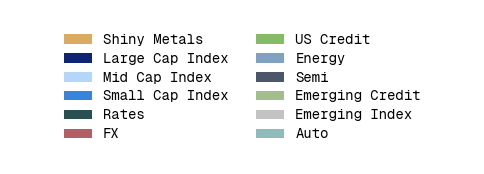
\includegraphics[width=0.8\textwidth]{images/ticker_color_code.png}
    \caption{Color coding for different asset classes}
    \label{fig:asset_class_colors}
\end{figure}
